\documentclass[a4paper, 14pt]{extarticle}%тип документа

%Русский язык
\usepackage[T2A]{fontenc} %кодировка
\usepackage[utf8]{inputenc} %кодировка исходного кода
\usepackage[english,russian]{babel} %локализация и переносы

%отступы 
\usepackage[left=2cm,right=2cm,top=2cm,bottom=3cm,bindingoffset=0cm]{geometry}

%Вставка картинок
\usepackage{graphicx}
\usepackage{wrapfig, caption}
\graphicspath{}
\DeclareGraphicsExtensions{.pdf,.png,.jpg, .jpeg}
\newcommand\ECaption[1]{%
     \captionsetup{font=footnotesize}%
     \caption{#1}}

%Таблицы
\usepackage[table,xcdraw]{xcolor}
\usepackage{booktabs}

%Графики
\usepackage{pgfplots}
\pgfplotsset{compat=1.9}

%Математика
\usepackage{amsmath, amsfonts, amssymb, amsthm, mathtools}

%Заголовок
\author{Подлесный Артём \\ группа 827}
\title{Работа 4.3.2Б \\ ДИФРАКЦИЯ СВЕТА НА УЛЬТРАЗВУКОВОЙ ВОЛНЕ В ЖИДКОСТИ}

\begin{document}
\maketitle

\paragraph*{Цель работы:} изучение дифракции света на синусоидальной акустической решётке и наблюдение фазовой решётки методом тёмного
поля.

\paragraph*{Оборудование:} оптическая скамья, осветитель, два длиннофокусных объектива, кювета с жидкостью, кварцевый излучатель
с микрометрическим винтом, генератор ультразвуковой частоты, линза, вертикальная нить на рейтере, микроскоп.

\section*{Краткая теория}

В работе изучается дифракция света на фазовой решётке. Фазовая
решётка создаётся в жидкости ультразвуковыми волнами и наблюдается методом тёмного поля.
\begin{wrapfigure}{l}{0.3\textwidth}
\begin{center}
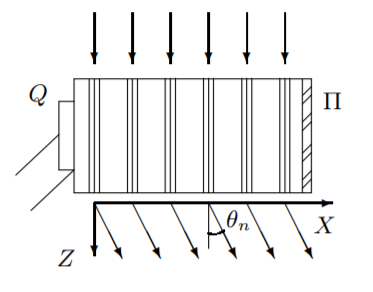
\includegraphics[height=4cm]{teor.png}
\end{center}
\ECaption{Дифракция световых волн
на акустической решётке}
\end{wrapfigure}
При прохождении ультразвуковой (УЗ) волны через жидкость
в ней возникают периодические оптические неоднородности, обусловленные разницей значений коэффициента преломления в областях
сжатия и разрежения. Эти периодические неоднородности играют
роль своеобразной дифракционной
решётки для проходящего сквозь
жидкость света.
При небольших амплитудах звуковой волны показатель преломления жидкости n меняется по закону:
\begin{equation}
n = n_0(1 = m\cos \Omega x),
\end{equation}
где $\Omega$ — волновое число для УЗ-волны $(\Omega = 2\pi/\Lambda)$, $\Lambda$ — длина УЗволны, $m$ — глубина модуляции показателя преломления, определяемая
интенсивностью ультразвуковой волны $(m \ll 1)$.

Пусть фаза световых колебаний на передней поверхности жидкости
равна нулю. Тогда на задней поверхности (т.е. в плоскости z = 0) она
равна
\begin{equation}
\varphi = knL = \varphi_0(1+m\cos\Omega x),
\end{equation}
где $L$ — толщина слоя жидкости в кювете, $k$ — волновое число для света $(k = 2\pi/\lambda)$, $\lambda$ — длина световой волны, $\varphi_0 = kn_0L$. Таким образом,
в плоскости $z = 0$ фаза световых колебаний является периодической
функцией координаты $x$, иными словами — УЗ-волна в жидкости создаёт фазовую дифракционную решётку. Условие, при котором можно рассматривать решетку как чисто фазовую, можно записать так:
\begin{equation}
m\ll \frac{\Lambda}{L}\sqrt{\dfrac{\lambda}{L}}.
\end{equation}
Таким образом, чисто фазовая акустическая решётка реализуется лишь
на достаточно слабой УЗ-волне. При повышении мощности ультразвука акустическая волна начинает работать как сложная амплитуднофазовая решётка.
В общем
случае после прохождения через кювету световое поле представляет
совокупность не трёх, а большого числа плоских волн, распространяющихся под углами, определяемыми условием
\begin{equation}
\Lambda\sin \theta_m = m\lambda, \text{ } (m = 0, \pm 1,...).
\end{equation}
Каждая из этих волн соответствует одному из максимумов в дифракционной картине Фраунгофера.
Определяя на опыте положение дифракционных максимумов различного порядка, можно по формуле найти длину $\Lambda$ УЗ-волны и
вычислить скорость $v$ распространения ультразвуковых волн в жидкости, если известна частота $\nu$ колебаний кварцевого излучателя:
\begin{equation}
v = \Lambda \nu.
\end{equation}


\section*{Экспериментальная установка}

\begin{figure}[h]
\begin{center}
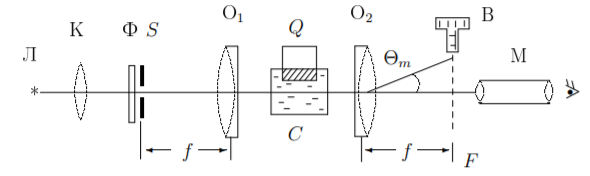
\includegraphics[width=0.9\textwidth]{ust}
\end{center}
\ECaption{Схема для наблюдения дифракции на акустической решётке.}
\end{figure}

В  силу
малости углов $\theta_m$ окончательное выражение может быть представлено
в виде
\begin{equation}
l_m = mf\frac{\lambda}{\Lambda},
\end{equation}
где $l_m$ — измеренное на опыте линейное расстояние между m-м и нулевым максимумами, а $f$ — фокусное расстояние объектива О2.

\section{Определение скорости ультразвука по дифракционной картине}

В работе предлагается измерить координаты дифракционных полос, образующихся при дифракции света на акустической решётке, а
также определить период этой решётки методом тёмного поля. По результатам измерений рассчитывается скорость ультразвука в воде. Все
измерения ведутся на стоячей волне. 

После настройки оборудования, была получена дифракционная картина. По ней, измерив по порядку длину УЗ-волны, как удвоенное расстояние между соседними дифракционными картинами, по (5) была измерена приблизительная скорость звука в воде. Результаты на таблице 1.

\begin{table}[h!]
\begin{center}
\begin{tabular}{|c|c|c|}
\hline
\rowcolor[HTML]{9698ED} 
$\lambda$, мкм   & $f$, MHz      & $v$, м/с    \\ \hline
690 & 1.111 & 1533 \\ \hline
\end{tabular}
\ECaption{}
\end{center}
\end{table}

Как видно, приближенное значение соответствует действительности, так как скорость звука в воде колеблется в районе 1500 м/с. 

После этого была проведена основная работа этого пункта, были определены положения дифракционных полос при разной рабочей частоте. Эти данные показаны на таблице 2:

\begin{table}[h!]
\begin{center}

\begin{tabular}{|c|c|c|}
\hline
\rowcolor[HTML]{9698ED} 
$f$, MHz & $Y$, дел & $m$  \\ \hline
\rowcolor[HTML]{9698ED} 
1.023  & 76     & 2  \\ \hline
       & 47     & 1  \\ \cline{2-3} 
       & 19     & 0  \\ \cline{2-3} 
       & -16    & -1 \\ \cline{2-3} 
       & -49    & -2 \\ \hline
\rowcolor[HTML]{9698ED} 
2.161  & 83     & 1  \\ \cline{2-3} 
       & 19     & 0  \\ \cline{2-3} 
       & -54    & -1 \\ \hline
\rowcolor[HTML]{9698ED} 
4.477  & 153    & 1  \\ \cline{2-3} 
       & 19     & 0  \\ \cline{2-3} 
       & -124   & -1 \\ \hline
\rowcolor[HTML]{9698ED} 
0.862  & 43     & 1  \\ \cline{2-3} 
       & 19     & 0  \\ \cline{2-3} 
       & -11    & -1 \\ \cline{2-3} 
       & -40    & -2 \\ \hline
\end{tabular}
\ECaption{Координаты дифракционных полос. Отмерены с помощью винта В. Один оборот - 100 делений, так что обороты так же учитывались. Все необходимые данные по цене деления представлены на установке.}
\end{center}
\end{table} 

Как видно, полос довольно мало, что связано с недостаточно хорошей настройкой установки. Для каждой из частот построен график, по которому можно определить рнасстояние между дифракционными полосами. График показан на рис 3.

\begin{figure}[h]
\begin{center}
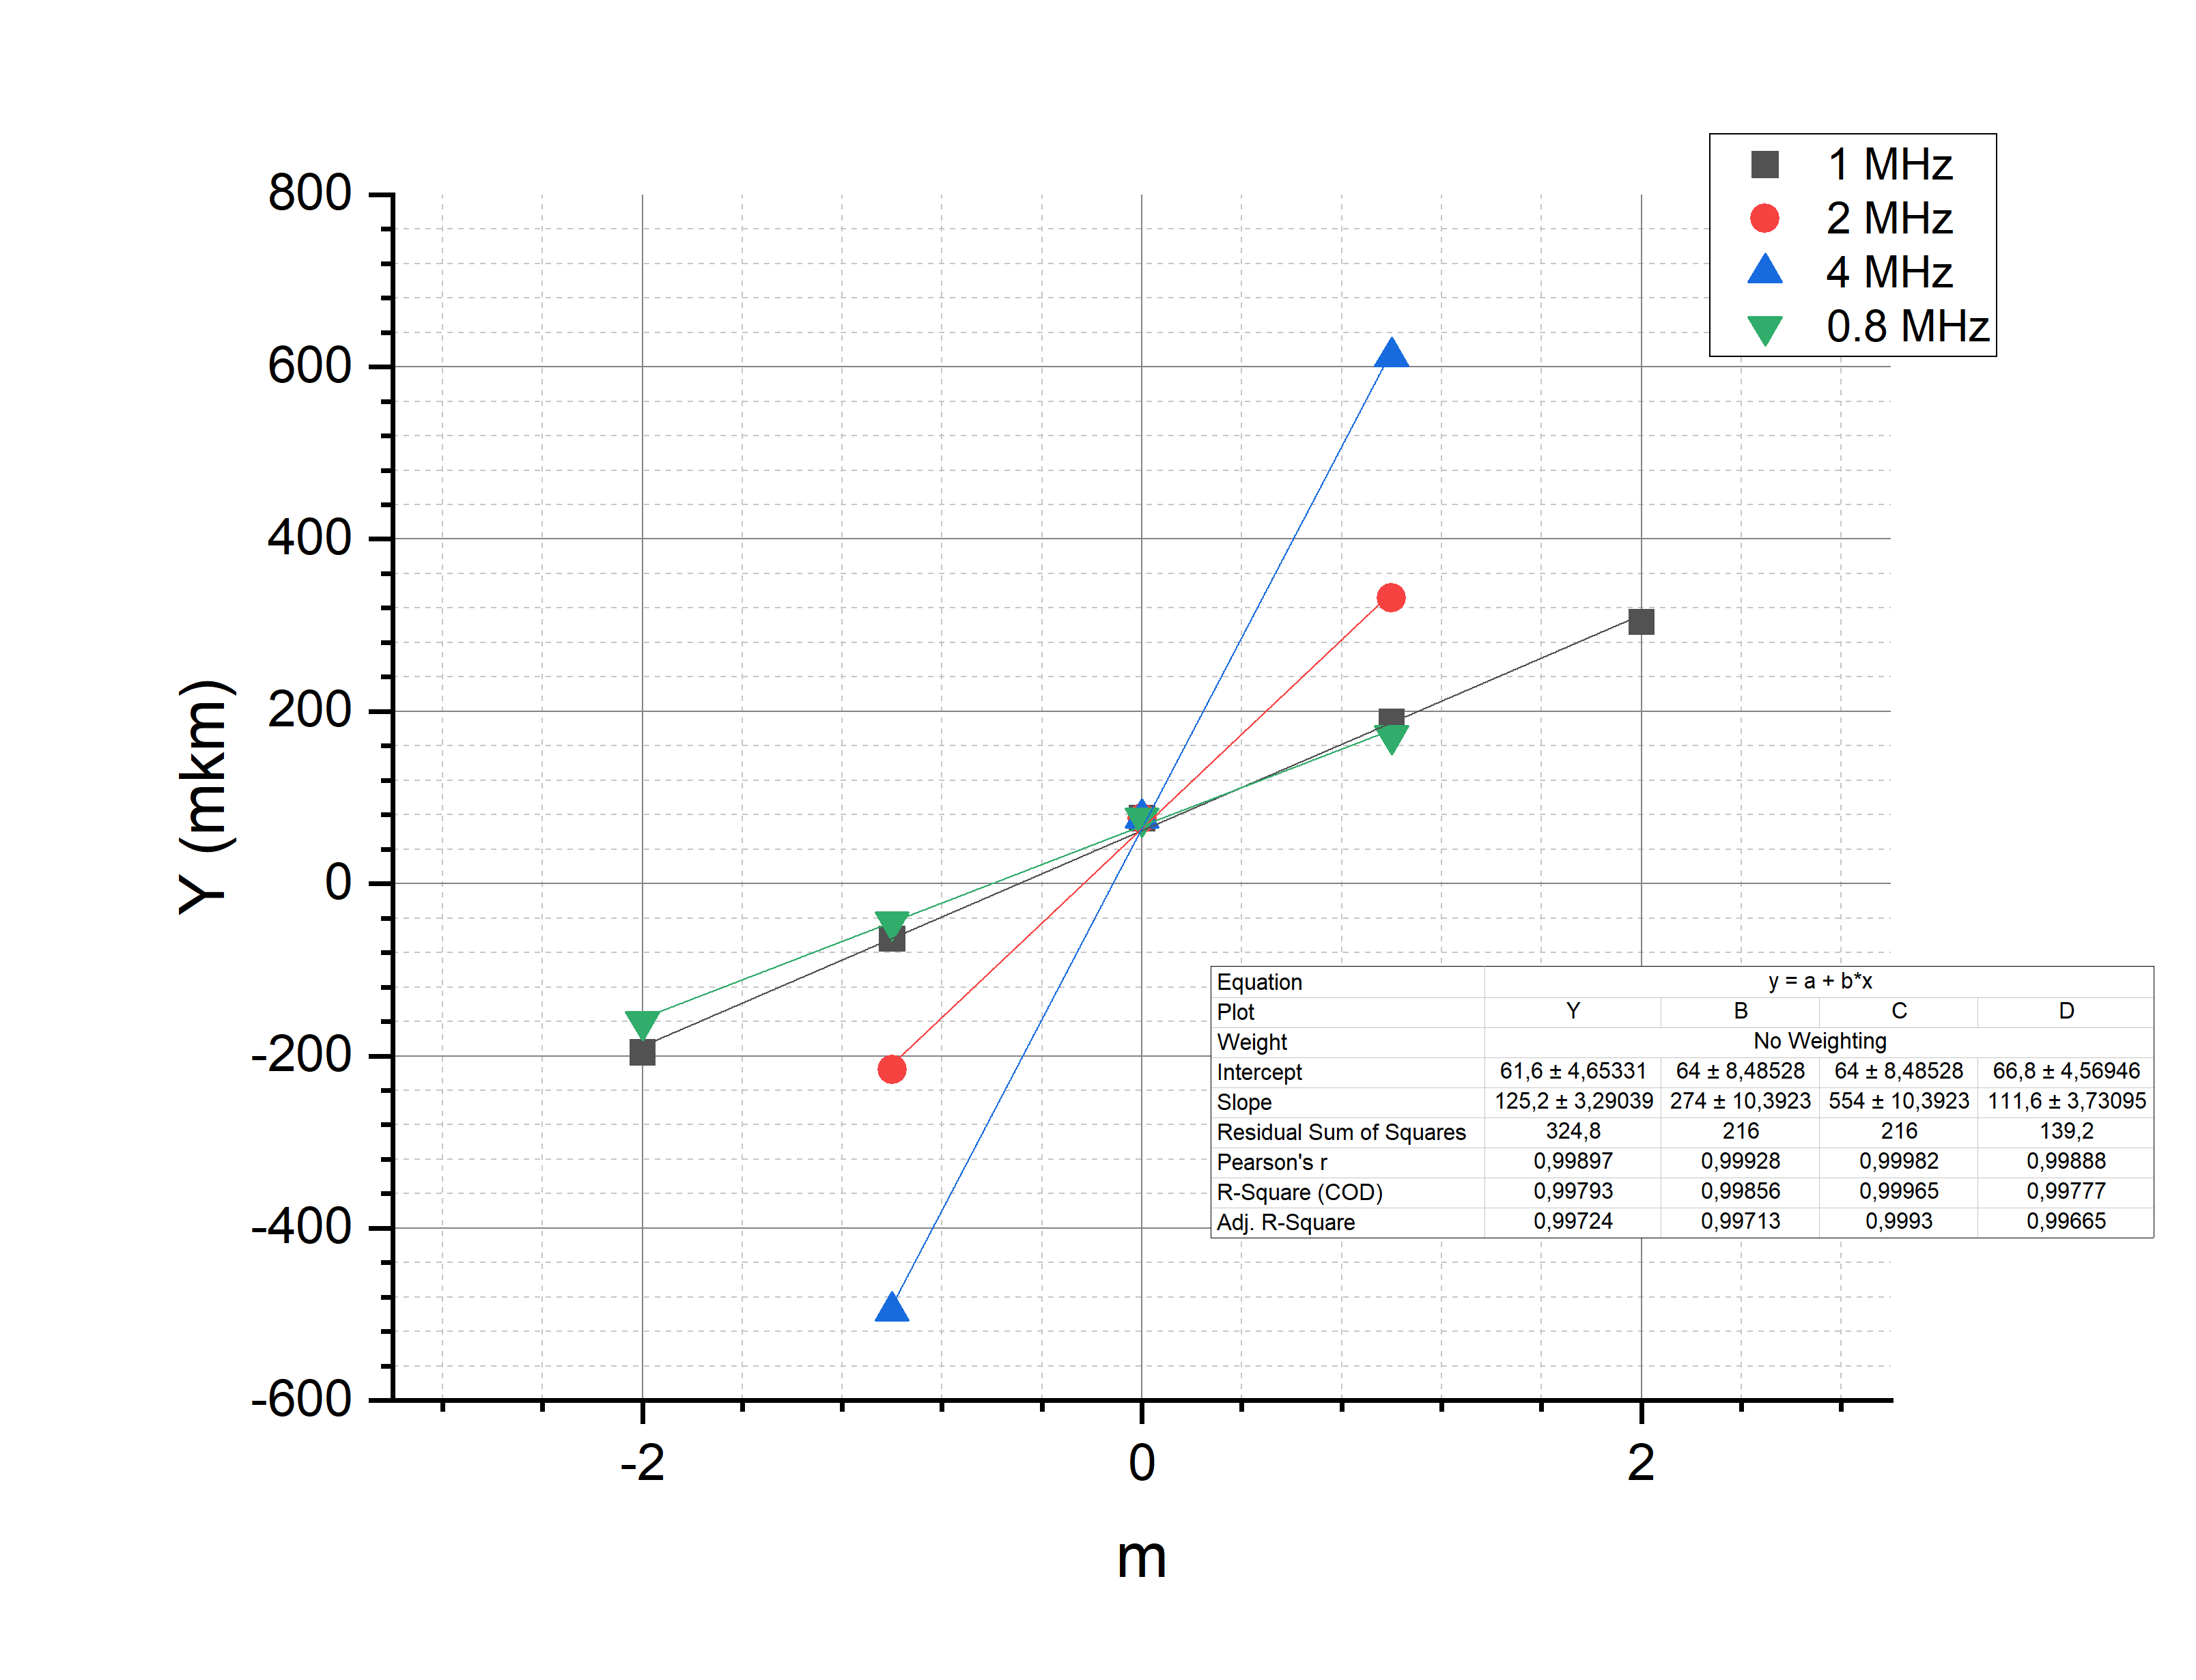
\includegraphics[width=0.9\textwidth]{gr1}
\end{center}
\ECaption{График зависимости $Y(m)$. Разными цветами обозначены графики для разных рабочих частот.}
\end{figure}

Таким образом получена зависимость длины УЗ волны $\Lambda$ от частоты с помощью формулы (6). На основе нее, с помощью формулы (5) получена зависимость скорости звука от рабочей частоты. Обе зависимости представлены на таблице 3.

\begin{table}[h!]
\begin{center}

\begin{tabular}{|c|c|c|c|c|c|c|}
\hline
\rowcolor[HTML]{9698ED} 
$f$, MHz    & $l$, мкм   & $\sigma_{l}$, мкм & $\Lambda$, cm      & $\sigma_{\Lambda}$, cm    & $v$, м/с       & $\sigma_v$, м/с    \\ \hline
0.862 & 112 & 4  & 160.00 & 10.71 & 1379.20 & 92.36 \\ \hline
\rowcolor[HTML]{9698ED} 
1.023 & 125 & 3  & 143.36 & 7.92  & 1466.20 & 81.01 \\ \hline
2.161 & 274 & 10 & 65.40  & 4.43  & 1413.63 & 95.77 \\ \hline
\rowcolor[HTML]{9698ED} 
4.477 & 554 & 10 & 32.35  & 1.59  & 1448.25 & 71.40 \\ \hline
\end{tabular}
\ECaption{Зависимости длин волн и скоростей звука в воде от частоты генератора. }
\end{center}
\end{table}

Данные вполне достоверны, тк близки к табличным значениям.

Средняя скорость звука в воде, полученная в работе, равна:
\[v_{\text{зв}} = 1427\pm86 \text{ м/с}.\]

\section*{Определение скорости ультразвука методом тёмного поля}

После настройки оборудования, когда был затемнен первый максимум, и была получена звуковая дифракционная картина, был проведен эксперимент. В зависимости от частоты измерялись координаты первой и последней хорошо видимых темных полос, а так же кол-во светлых между ними. На основании этого можно определить $\Lambda$. Данные на таблице 4.

\begin{table}[h!]
\begin{center}

\begin{tabular}{|c|c|c|c|c|}
\hline
\rowcolor[HTML]{9698ED} 
f MHz & Y1 & Y2  & N  & l      \\ \hline
2.168 & 5  & 150 & 18 & 64.44  \\ \hline
\rowcolor[HTML]{9698ED} 
4.430 & 23 & 125 & 26 & 31.38  \\ \hline
1.552 & 20 & 120 & 9  & 88.89  \\ \hline
\rowcolor[HTML]{9698ED} 
1.178 & 30 & 105 & 5  & 120.00 \\ \hline
\end{tabular}
\ECaption{Экспериментально, при помощи метода темного поля, определенная длина УЗ волны в зависимости от частоты.}
\end{center}
\end{table}

Осталось лишь определить скорость звука из соответствующего графика, представленного на рис 4.

\begin{figure}[h]
\begin{center}
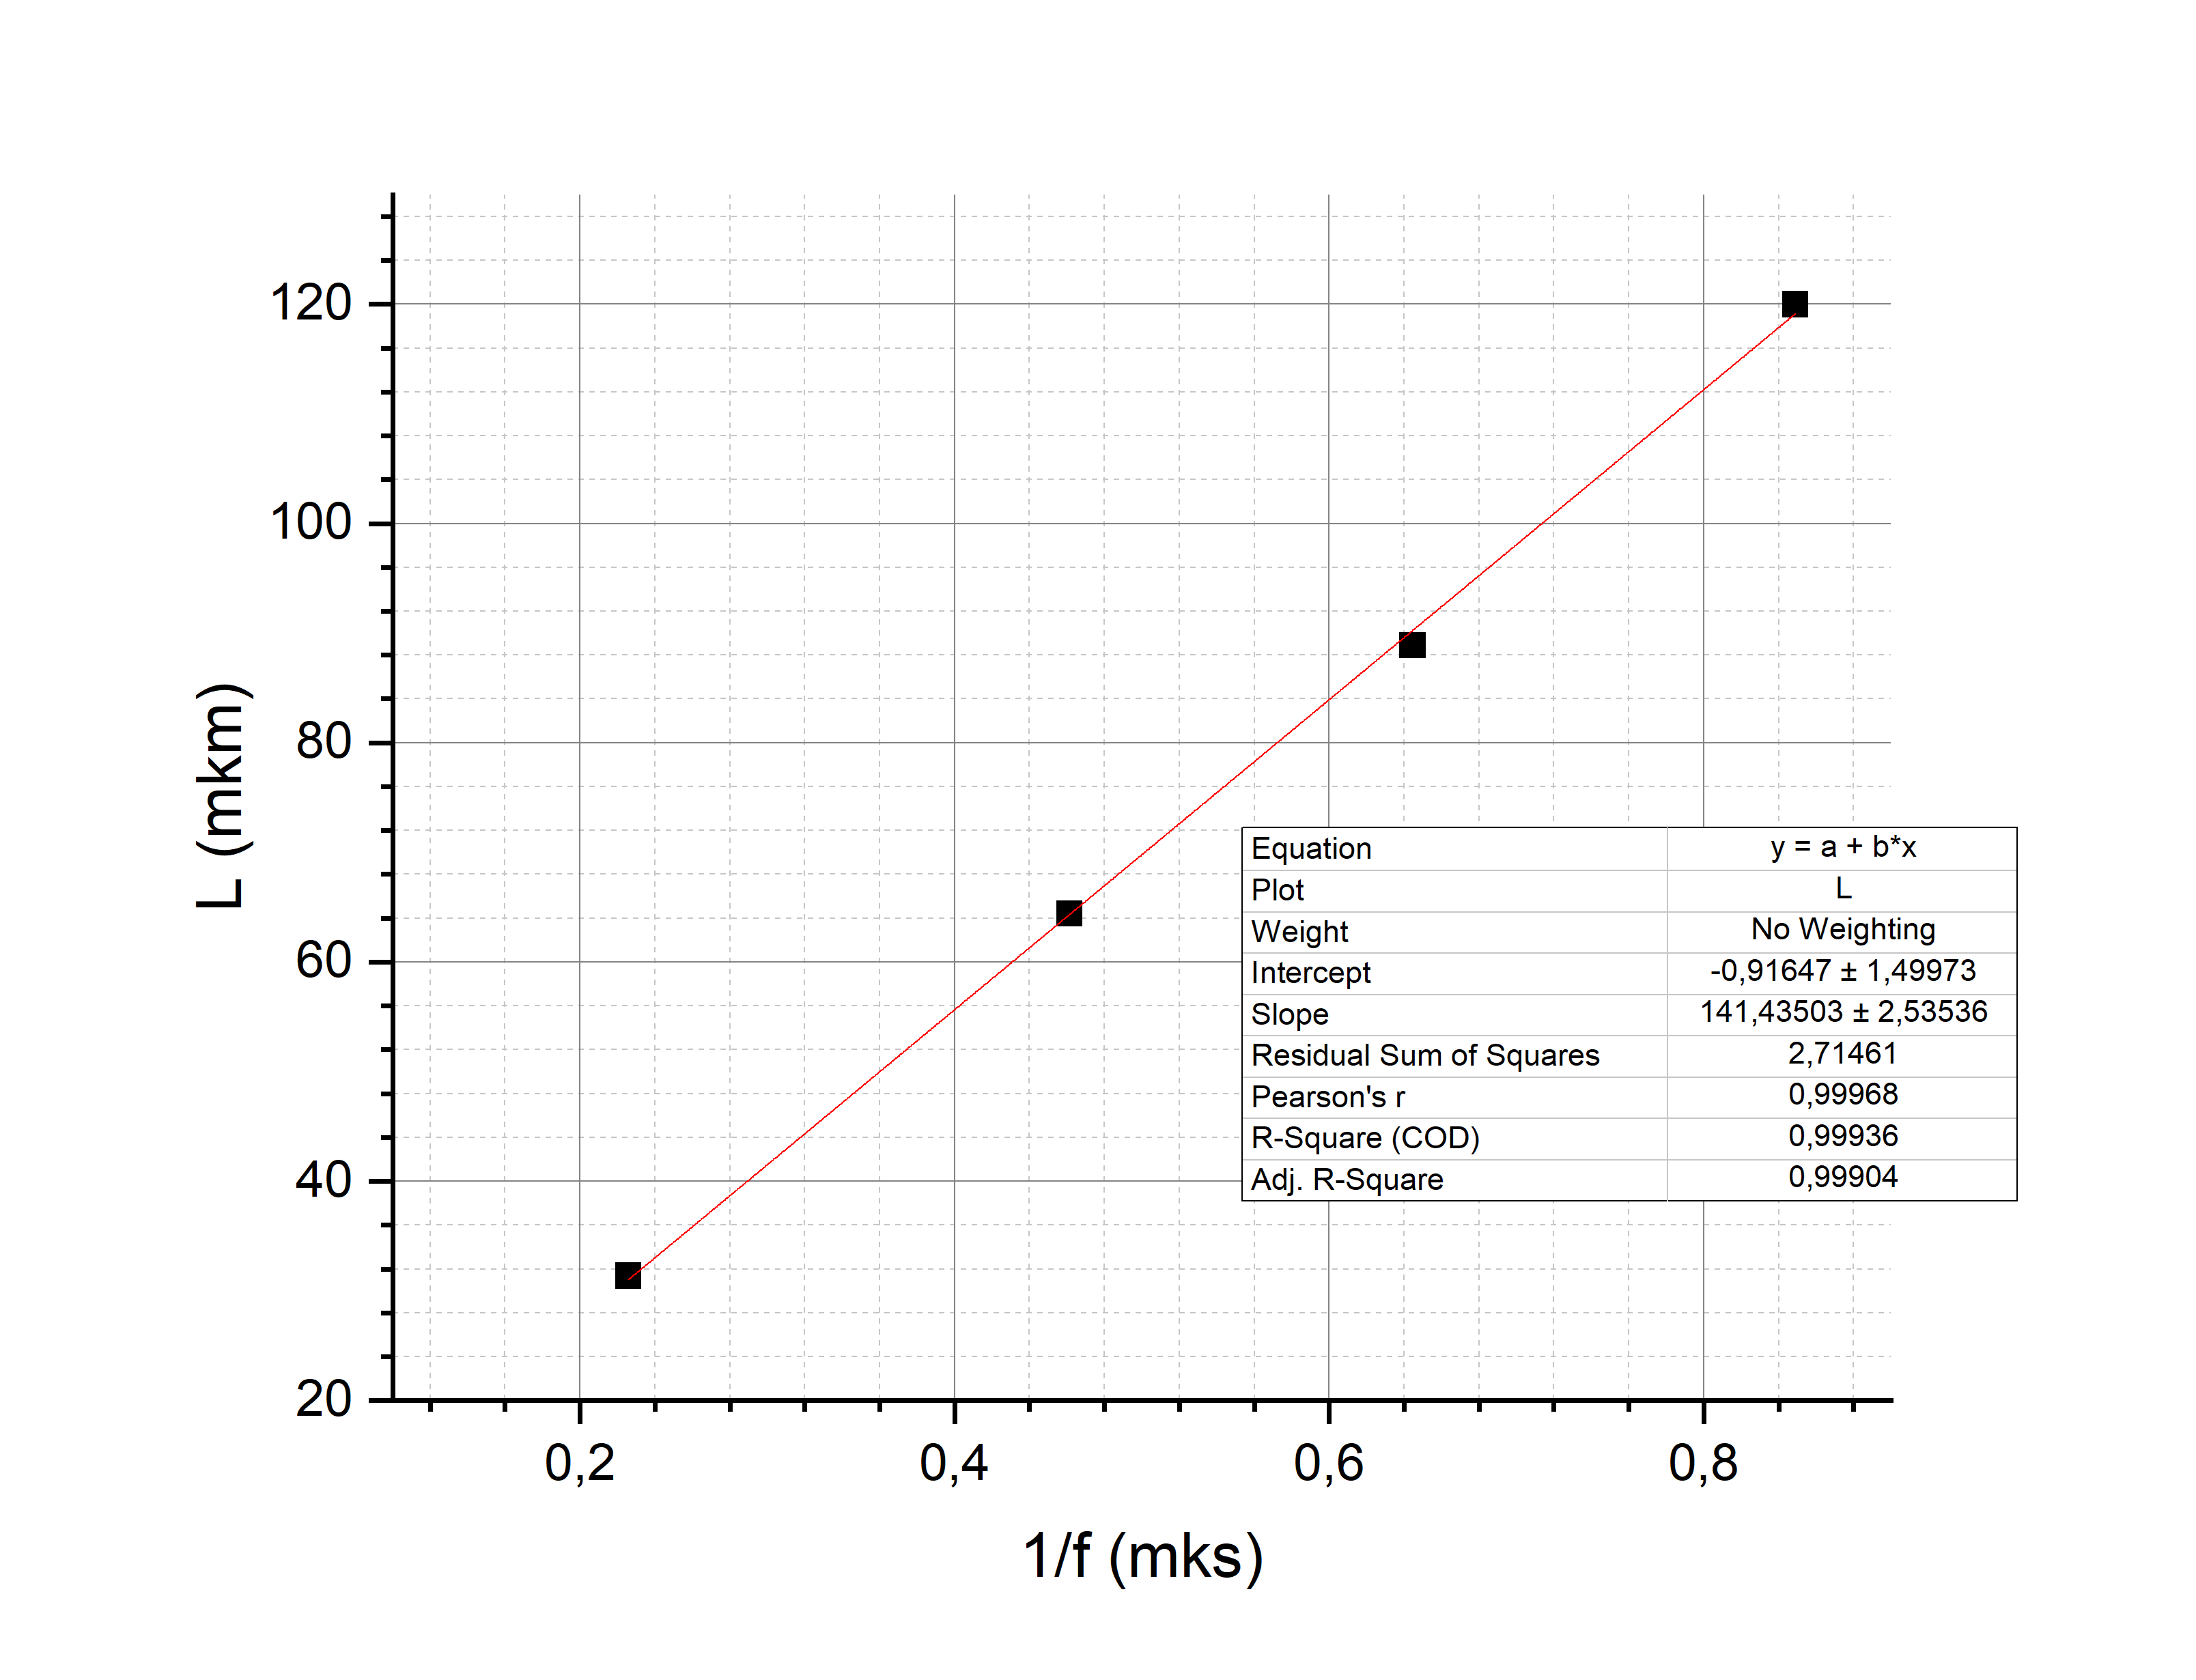
\includegraphics[width=0.9\textwidth]{gr2}
\end{center}
\ECaption{График зависимости $\Lambda(\frac{1}{\nu})$. Хоть он и построен по 4 точкам, но я им горжусь. Так, в целом, выглядят все графики в этой работе.}
\end{figure}

Из коэффициента наклона находим значение для скорости ультразвука в воде:
\[v = 1414 \pm 25 \text{ м/с}. \]
Однако погрешность этого значения не до конца соответствует действительности, так как при непосредственном измерении кол-ва светлых полос можно было легко обсчитаться. К тому же границы дифр решетки были достаточно размыты, так что не было четкого критерия для определения $Y_1$ и $Y_2$. Тем не менее результаты двух методов вполне согласуются. 
 
\section*{Вывод}
Была изучена дифракция света на синусоидальной акустической решетке, и фазовая решетка наблюдалась методом темного поля. В ходе работы скорость ультразвука в воде была определена двумя способами: по дифракционной картине и методом темного поля. Полученные этими способами результаты совпали с хорошей точностью. Недостаток возможности получения большего кол-ва данных связан прежде всего с не совсем точной настройкой оборудования, что, в свою очередь, связано с недостатком опыта у студентов в работе с оптикой.


\end{document}